% Template for ApJ-type papers

\documentclass[iop,twocolappendix]{emulateapj}

\usepackage{rotating}
\usepackage{amssymb,amsmath}
\usepackage{graphicx}%[subfloat]
\usepackage{natbib}
\usepackage{float}
\usepackage{subfig}
\usepackage{multirow}
\usepackage{subcaption}
\citestyle{aa}
\bibliographystyle{apj_w_etal}

\newcommand{\vect}[1]{\mathbf{#1}}
\newcommand{\xad}{\vect{x}}

\newcommand{\vdag}{(v)^\dagger}
\newcommand{\myemail}{jaguirre@nrao.edu}
\newcommand{\lsim}{{_{<}\atop^{\sim}}}
\newcommand{\gsim}{{_{>}\atop^{\sim}}}
\newcommand{\etal}{{et al.\/}}
\newcommand{\ie}{{\em ie.\/}}
\newcommand{\cmq}{cm{$^{-3}$}}
\newcommand{\per}{$^{\rm{-1}}$}
\newcommand{\tc}{{$\theta^1$~Orionis~C}}
%\newcommand{\msol}{M{$_{\odot}$}}
%\def\msol{\ifmmode {\>M_\odot}\else {$M_\odot$}\fi}
\newcommand{\lsol}{L{$_{\odot}$}}
\newcommand{\kms}{km~s{$^{-1}$}}
\newcommand{\hii}{H~{\sc ii}}
\newcommand{\Hii}{H~{\sc ii}}
\newcommand{\Ha}{\mbox{H$\alpha$}}
\newcommand{\sii}{S~{\sc ii}}
\newcommand{\Feii}{Fe~{\sc ii}}
\newcommand{\oi}{O~{\sc i}}
\newcommand{\nii}{N~{\sc ii}}
\newcommand{\oiii}{O~{\sc iii}}
\newcommand{\mgii}{Mg~{\sc ii}}
\newcommand{\tco}{{$^{13}$CO}}
\newcommand{\CO}{{$^{12}$CO}}
\newcommand{\Tco}{{$^{12}$CO}}
\newcommand{\co}{C{$^{18}$O}}
\newcommand{\Lsol}{L$_{\odot}$}
\newcommand{\Msol}{M$_{\odot}$}
%\newcommand{\C18o}{C$^{18}$O($1\rightarrow 0$)}
%\newcommand{\Check}{{\bf ???}}
\newcommand{\mum}{\ensuremath{\mu \mathrm{m}}}
\newcommand{\flux}{flux density}
\newcommand{\solar}{\ensuremath{\odot}}

\newcommand{\epsi}{\varepsilon}
\newcommand{\herschel}{{\em Herschel}}


\newcommand{\TBD}{{\bf TBD}}

%\def\Figure#1#2#3#4{
%\begin{figure}[htb]
%\epsscale{#4}
%\plotone{#1}
%\caption{#2}
%\label{#3}
%\end{figure}
%}

%\def\Table#1#2#3#4#5{
%\begin{deluxetable}{#1}
%\tablewidth{0pt}
%\tablecaption{#2}
%\tablehead{#3}
%\startdata
%\label{#4}
%#5
%\enddata
%\end{deluxetable}
%}

\newcommand{\cii}{[C{\sc ii}]}
\def\hi{H{\sc i}}
\newcommand{\smg}{SMG}
\newcommand{\smgs}{SMGs}

\newcommand{\penn}{1}
\newcommand{\jpl}{2}
	% End definitions


\shorttitle{[CII] Line Intensity Mapping During $0.5 < \Makelowercase{z} < 1.5$}
\shortauthors{Uzgil, Aguirre \& Bradford}

\begin{document}

\title{Measuring galaxy clustering and the evolution of [CII] mean intensity with Far-IR line intensity mapping during $0.5 < \MakeLowercase{z} < 1.5$}

\author{B.~D.~Uzgil\altaffilmark{\penn,\jpl}}

\author{J.~E.~Aguirre\altaffilmark{\penn}}

\author{C.~M.~Bradford\altaffilmark{\jpl}}

\email{badeu@sas.upenn.edu}

\altaffiltext{\penn}{University of Pennsylvania, Philadelphia, PA 19104}

\altaffiltext{\jpl}{Jet Propulsion Laboratory}

\begin{abstract}

Infrared fine-structure emission lines from trace metals are powerful diagnostics of the interstellar medium in galaxies. We explore the possibility of studying the redshifted far-IR fine-structure line emission using the three-dimensional (3D) power spectra obtained with an imaging spectrometer.  The intensity mapping approach measures the spatio-spectral fluctuations due to line emission from all galaxies, including those below the individual detection threshold. The technique provides 3D measurements of galaxy clustering and moments of the galaxy luminosity function.  Furthermore, the linear portion of the power spectrum can be used to measure the total line emission intensity including all sources through cosmic time with redshift information naturally encoded.   Total line emission, when compared to the total star formation activity and/or other line intensities reveals evolution of the interstellar conditions of galaxies in aggregate.  As a case study, we consider measurement of [CII] autocorrelation in the $0.5 < z < 1.5$ epoch, where interloper lines are minimized, using far-IR/submm balloon-borne and future space-borne instruments.  In this context, we compare the intensity mapping approach to blind galaxy surveys based on individual detections.  We find that intensity mapping is nearly always the best way to obtain the total line emission because galaxy surveys lack either depth or sufficient volume to overcome cosmic variance.  Even if absolute mean intensity is not desired, intensity mapping is often the most efficient way to measure the power spectrum shape, depending on the details of the luminosity function and the telescope aperture.

\end{abstract}

\keywords{far-infrared spectroscopy; galaxy redshift surveys}

%18:11 Pacific 7/20/2013

% - Section 2, in which we discuss the model used for predicting the line power spectra, remains relatively unscathed. Need to keep discussion of lines general, and refrain from using [CII] as a specific example here. Also, will add an intro to the cross power spectrum and the theoretical explanation of the problem of interloper lines at the end of this section.
% 
% - Section 3, the "observational strategy section". Figure 2 will be moved to later in the section. Figures 4, 5, 8 -- the mode counting and SNR vs k plots -- will moved to the beginning. Figure 4 will be changed so that the left-hand point is (0,0) and the k_par and k_perp axes are equal in length. That way, we can identify "k-parallel" or "k-perpindicular" dominated modes as above and below a line drawn at 45 degrees from the origin. We can also plot the region affected by foreground contamination in the k_par-k_perp plane. Figures 6 will be redone to show that with 450 hours, one can measure the [SiII] power spectrum from individually detected sources, but with 45 hours, it is no longer possible to do so, while there is still high S/N on the intensity mapping measurement. We will include a new table that shows the Figure of Merit for the other lines, answering the question "At what z and with which lines is intensity mapping more efficient?"
% 
% - Need to mention that selecting a line is effectively selecting a galaxy type (e.g. high ionization lines for AGN) and so measuring different clustering with the different lines has astrophysical implications. (Are there any references to support why this might be expected to happen, beyond the old "red vs blue" galaxies observation? Thinking off the top of my head, I can imagine it might be possible to detect a different clustering signal for galaxies that are primarily found in merging systems. Not sure how big of an affect this would be in the power spectrum...)
% 
% -Figure 10 needs to make a new point. That is, we must show that the choice of Bethermin model here is robust enough to make valid predictions, based on what is already measured from the cosmic star formation history (Hopkins+Beacom). Also need to show that for lines that have a deficit with respect to LIR and and have a steep LF at the bright end, intensity mapping is useful. (But we have to be careful because [SiII] does not have this deficit with LIR and we have shown intensity mapping to be useful for this line.)

\section{Introduction}

Line intensity mapping, or 3-D tomographic mapping, allows astronomers to probe extragalactic light from all sources, including the faintest galaxies and even diffuse intergalactic emission. An intensity mapping survey of a spectral line at different frequencies produces a fully three dimensional data cube containing ``tomographic scans" of the Universe along the spectral (i.e., redshift) direction. The spatial fluctuations in line emission, contained in the data cube, are then decomposed into the power spectrum. Atomic \citep{gongcii,visbal11} and molecular \citep{lidz11,gong11co} transitions -- such as the 21-cm spin flip transition from H$^{\mathrm{o}}$, CO (2-1), and [CII]158$\mu$m -- have been investigated as candidates for intensity mapping experiments during the Epoch of Reionization (EoR). Of these, the neutral hydrogen case is undoubtedly the most developed in terms of its standing in the literature (cf. \citet{morales10rev} for a review) and in the experimental arena (e.g., PAPER \citep{parsons14}, MWA \citep{tingay13}) because intensity mapping is the only means of studying the intergalactic HI light. [CII] later emerged as an EoR intensity mapping candidate since it both offers a way to probe the clustering of sources from the faint-end of the luminosity function, and provides an opportunity for cross-correlation with the HI datasets \citep{gongcii}.

Aside from tracing large-scale structure, [CII] also contains astrophysical information about the conditions in star-forming galaxies. With an ionization potential of 11.6 eV, it arises in both ionized and neutral atomic gas.  Empirically, it is an important coolant, often the brightest single line in the spectrum of a star-forming galaxy, emitting as much as 0.5--1\% of the total FIR luminosity \citep{malhotra97,luhman98,stacey10,graciacarpio11}.   The ratio of the [CII] luminosity to the total bolometric luminosity can be used as a diagnostic tool that provides: (1) a measure of the star-formation activity, (2) a measure of the spatial extent (or ``mode") of star formation, and (3) an AGN/starburst discriminant \citep{hailey-dunsheath10,stacey10,graciacarpio11,sargsyan12,diaz-santos13}.

The broader suite of far-IR lines probes all phases of the interstellar medium, and the negligible optical depth of galaxies at far-IR wavelengths ensures that even the most heavily embedded regions where stars form and black holes grow are revealed. For the atomic and ionized medium, the key far-infrared emission lines are those of C, N, \& O (e.g., [OI]63$\mu$m, 146$\mu$m, [CII]158$\mu$m, [OIII]52$\mu$m, 88$\mu$m, [NIII]57$\mu$m, and [NII]122 $\mu$m, 205 $\mu$m). The emitting species cover more than an order of magnitude in ionization potential and they strongly constrain the density and temperature of the ionized and neutral gas, and the strength and hardness of the interstellar radiation field.  These physical parameters then reveal the relative importance of the black hole vs. the hot young stars to the overall energy budget, and constrain the stellar effective temperatures \cite[e.g.]{rubin85,dale04,colbertM82,malhotra01,ferkinhoff11,lebouteiller12}. The suite of carbon, oxygen and nitrogen transitions also measure abundances \citep{garnett04, lester87,nagao11}.

A power spectrum analysis of 3D tomography using the far-IR fine structure lines would expand upon recent works that utilize the fluctuations in emission rather than individual object detections to study the properties of dusty, star-forming galaxies (DSFGs) with continuum data. These studies, using \emph{P(D)} \citep{glenn10, bethermin11} or a 2-D power spectrum \citep{viero13, planckXXX} analysis, have already shed light on some aspects (such as galaxy number counts, spatial clustering, and cosmic evolution of IR luminosity density) of the bulk of these systems during the peak of cosmic star formation, but they are limited by source confusion or uncertainties associated with the lack of redshift information. Redshift ambiguities can be removed to some extent with galaxy-by-galaxy observations with the interferometers ALMA or NOEMA, or with an instrument like X-Spec, a proposed multi-object spectrometer for CCAT. However, the interferometer surveys will be expensive and will cover very little sky, and the CCAT surveys, though faster, will not reach the faintest galaxies in the luminosity function \citep{bradford09ccat}. Power spectrum treatment of the 3-D datasets naturally combines the redshift precision of spectral measurements, while including all sources in the luminosity function, and can be carried out with an instrument that does not require exquisite point-source sensitivity. 

%This sensitivity of the line intensity mapped power spectrum to galaxies below the individual detection threshold, indeed to the mean aggregate intensity in the line from all sources, is a unique line of inquiry for the galaxy populations. An example of using the power spectrum to determine luminosity density can be found in \citet{planckXXX}, although the results discussed there were derived from the 2-D angular power spectrum of IR continuum fluctuations, which relies on fits which include uncertainties in the dust spectral energy distributions, for instance. With inherent redshift information from the spectral line, such an observation of the 3-D power spectrum would ascertain the cosmic evolution of the Universe's total output in a given line with a level of precision not available by other means. 

Line intensity mapping experiments targeting the fine structure metal lines at post-Reionization redshifts can offer a proof of principle of the approach, similar to measurements of the HI autocorrelation power spectrum at $z\sim0.8$ \citep{chang10, switzer13}, and provide a complete census of galaxies during an important phase in the star formation history of the Universe. While the redshifted far-IR lines are not accessible from the ground in this redshift range, a balloon- or space-borne intensity mapping experiment with broad wavelength coverage could in principle measure the mean intensities of these lines through cosmic time, thereby charting the evolution of the star-formation conditions in galaxies in an absolute, aggregate sense.   Here we consider a first step in this direction, a measurement of [CII] autocorrelation in multiple bins through the $0.5 < z < 1.5$ epoch.   [CII] and far-IR lines in general ought to be particularly well-suited to this time frame, as $z\sim1.5$ is believed to be the peak in the dust attenuation in galaxies, when roughly 80\% of the cosmic star formation rate density is obscured and captured only in the infrared emission of re-processed starlight by dust grains \citep{burgarella13}.   From a practical standpoint, [CII] in this epoch is relatively free of interloper lines, as we will see.

The organization of this paper is as follows. We have estimated the mean intensity for a suite of fine structure IR emission lines, including the [CII] line, based on empirical IR luminosity functions and line-to-IR luminosity correlations, and present these results in the context of a power spectrum model in Section 2. In Section 3, we envision suitable platforms for conducting the [CII] intensity mapping experiment and discuss the feasibility of detecting the [CII] power spectra in terms of the signal-to-noise ratio (SNR). From the power spectra, we provide estimates for accuracy in measuring the mean [CII] intensity as a function of redshift. To better assess the value of intensity mapping studies in the case of [CII] at moderate redshifts, and of intensity mapping experiments in general, we compare in Section 4 the performance of the intensity mapping approach against spectroscopic galaxy surveys that rely on individual detections of sources to measure the total emission and power spectrum. In particular, we examine the effects of variations in luminosity function shape, aperture diameter (and, consequently, voxel size), and experimental noise on the ability of each observational method to measure the power spectrum and provide a complete view of the galaxy population. 

\section{Predictions for FIR Line Power Spectra}

\subsection{Relationship Between Galaxy Populations and Fluctuation Power}

The complete autocorrelation power spectrum of a given far-IR fine structure line $i$ as a function of wavenumber $k$, $P_{i,i}(k,z)$, can be separated into power from the clustering of galaxies, $P_{i,i}^{clust}(k,z)$ and a Poisson term arising from their discrete nature, $P_{i,i}^{shot}(z)$. We compute the full nonlinear matter power spectrum, $P_{\delta,\delta}(k, z)$, using the publicly available code HALOFIT+ (http://camb.info), which has been the standard tool for predicting matter power spectra upon its success in fitting state-of-the-art dark matter simulations over a decade ago \citep{halofit}.  The clustering component of the line power spectrum is then written as

\begin{equation}
 P_{i,i}^{clust}(k, z) = \bar{S}_{i}^2(z) \bar{b_i}^2(z) P_{\delta\delta}(k, z).
 \label{eq:pclust}
 \end{equation}

Here we have implicitly assumed that the fluctuations in line emission trace the matter power spectrum with some average bias, $\bar{b_i}(z)$. For our target redshift range, $\bar{b}_i$ is reasonably well-constrained to be between 2 and 3.\citep{Cooray10, Jullo12}, so we have assumed a single bias at each redshift, although a more sophisticated model would allow for variation of the source bias with the host halo mass (and thus luminosity). 

The mean line intensity, $\bar{S}_{i}(z)$, in units of Jy sr$^{-1}$, can be calculated as

\begin{equation}
\bar{S}_{i}(z) = \int{\mathrm{d}n_{i} \frac{L_{i}}{4\pi D_L^2}} y_i D_A^2 ,
\label{eq:si}
\end{equation}

where the integration is taken with respect to $n_{i}$, the number of galactic line emitters per cosmological comoving volume element. The factor $y_i$ is the derivative of the comoving radial distance with respect to the observed frequency, i.e. $y = d\chi/d\nu = \lambda_{i,rest} (1+z)^2/H(z)$, and $D_A$ is the comoving angular distance.

Finally, the shot noise component of the total line power spectrum---with the same units as the clustering term, namely, Jy$^2$ sr$^{-2}$ (Mpc h$^{-1})^{3}$---takes the form 

\begin{equation}
P_{i,i}^{shot}(z) = \int{\mathrm{d}n_{i} \left( \frac{L_{i}}{4\pi D_L^2} \right)^2 \left( y_i D_A^2 \right)^2}.
 \label{eq:pshot}
\end{equation}

\subsection{Calculating IR line volume emissivity}

The number density of line emitters and the line luminosity that appear in equations (2) and (3) can be derived by a variety of methods. In earlier papers on intensity mapping of molecular and fine-structure emission lines at high redshift (z $\gtrsim$ 6), one approach involved using the dark matter halo mass function in lieu of the line emitter density (and invoking a one-to-one correlation between halos and galaxies, which is reasonable at high redshifts). The line luminosity, in turn, could be scaled according to the star formation rate, which was related to halo mass via a proportionality constant comprised of factors describing the fraction of baryons available for star formation, as well as the dynamical timescale for star formation and a duty cycle for emission. While this approach is perhaps justified for the very early Universe (given the lack of information about the galaxy luminosity function at high redshift), the situation at later times is better understood; we make use of empirical constraints on the $z\sim1$ epoch from FIR/submm number counts and observations of FIR line emission in galaxies. 

We first employ the empirically-constrained, backwards-evolution model of the IR luminosity function $\Phi(L_{IR}, z)$ from \citet{bethermin11} (hereafter B11) to predict the number of galaxies with luminosity $L_{IR}$ at a given redshift in some comoving volume of the Universe per logarithmic luminosity interval, i.e., $\frac{\mathrm{d}N(L_{IR},z)}{\mathrm{d}V\mathrm{dlog_{10}}L_{IR}}$ or $\frac{\mathrm{d}n_{IR}}{\mathrm{dlog_{10}}L_{IR}}$. 

To convert the infrared luminosity to a line luminosity, we apply the relation for $L_{i}$ as a function of $L_{IR}$ provided by \citet{spinoglio12}. (Working directly from the IR luminosity function, we do not include the population of IR-dark or IR-faint sources that nevertheless have bright emission in the far-IR fine structure lines (cf. \citet{Riechers14}).) The fit in their paper was based on the collection of ISO-LWS observations of local galaxies in \citet{brauher08}. For example, we reproduce below the relation for [CII]:

\begin{equation}
\mathrm{log_{10}}L_{\mathrm{[CII]}} = (0.89 \pm 0.03) \mathrm{log_{10}}L_{\mathrm{IR}} - (2.44 \pm 0.07),
\end{equation}

indicating that [CII] is suppressed for higher luminosity systems. The choice of using local $L_i$-$L_{IR}$ relations for our study of $z\sim1$ emitters may be unrealistic due to findings that suggest the so-called ``deficit" in [CII] and other FIR lines evolves with redshift such that the high-z counterparts to local systems do not exhibit suppressed FIR line emission. The local IR relations then can be interpreted as underestimating emission of the fine structure lines, since we likely overestimate the deficiency in the higher redshift, high luminosity systems of our model. While we use the combined Bethermin-Spinoglio model to predict line intensities and adopt it as our fiducial model throughout this paper, we hedge our predictions between estimates based on the cosmic star formation rate density as measured by \citet{hb06}. Furthermore, in Section 4 we explore variations in the shape of the IR luminosity function and consider an alternative line-to-IR luminosity ratio.

Next, it becomes possible to write the cosmic mean intensity and shot noise of the line, in units of Jy sr$^{-1}$,  as a function of redshift based on the B11 luminosity function and \citet{spinoglio12} $L_{i}-L_{\mathrm{IR}}$ relation as

\begin{equation} \label{eq:intensity}
\bar{S}_{\mathrm{i}}(z) = \int_{L_{IR,min}}^{L_{IR,max}} \mathrm{dlog}L_{IR}  \Phi(L_{IR}, z) \frac{f_{i} L_{IR} }{4 \pi D_{L}^2} y D_A^2
\end{equation}

\begin{equation} \label{eq:pshotlum}
P_{i,i}^{shot}(z) = \int_{L_{IR,min}}^{L_{IR,max}} \mathrm{dlog}L_{IR}  \Phi(L_{IR}, z) \left(\frac{f_{i} L_{IR}}{4 \pi D_{L}^2} y D_A^2\right)^2
\end{equation}

where $f_{i}$, i.e. $\frac{L_{i}(L_{IR})}{L_{IR}}$, is the fraction of IR luminosity emitted in line $i$, as computed from equation (3). In other words, we have written $\bar{S}_{i}$ and $P_{i,i}^{shot}(z)$ as the first and the second moments of the luminosity function.

\begin{figure}[t]
 \centering
 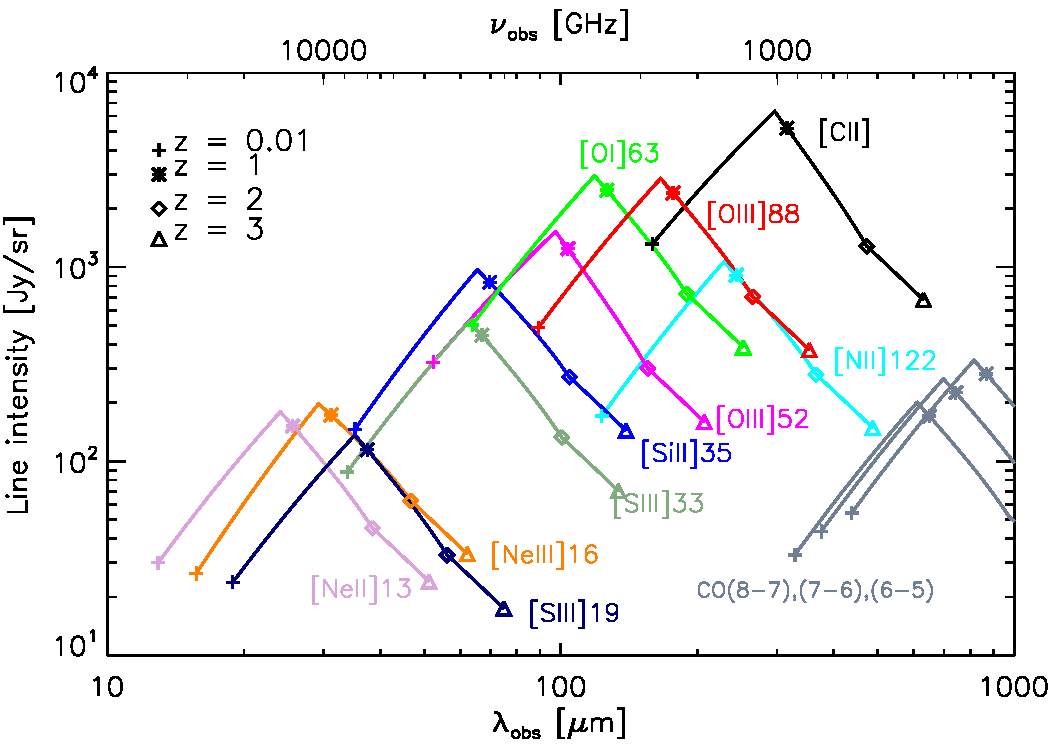
\includegraphics[width=0.45\textwidth]{interloper_intensity_jysr_withM82CO}
\caption{Intensity of fine structure line emission as a function of observed wavelength for the empirical model based on the B11 luminosity function. Intensities of CO lines, which are not included in the IR luminosity relations from \citet{spinoglio12}, have been estimated using a luminosity scaling provided by \citet{carilli11} for CO(1-0) and the relative intensities of the higher-J lines in \citet{bothwell13}.}
\label{fig:interlopers}
\end{figure}

The resulting mean intensities for a variety of FIR lines are plotted in Figure~\ref{fig:interlopers} as a function of redshift and observed wavelength. $\bar{S}_{i}$ vs $\lambda_{obs}$ can be interpreted as identifying the dominant source of fluctuations, according to our model, of a given wavelength. As a specific example, if the target line of an observation is [OI]63$\mu$m at $z = 1$, it is necessary to distinguish between the target line and interlopers like [OIII]88$\mu$m from $z=0.4$ and [OIII]52$\mu$m from $z=1.4$, which contribute power at the observed wavelength. \citet{visbal10} showed how the cross spectra can be used to differentiate between a target line and a contaminating line (or ``bad line", in their words), since emitters at different redshifts will be spatially uncorrelated. For the observed wavelengths of [CII], however, it is apparent from Figure 2 that, with the exception of contributions from [OIII]88$\mu$m and CO(8-7) near [CII] at $z \sim 0.01$ and $z>2$, respectively, the [CII] line is relatively unaffected by interloper lines---a result of its luminosity and spectral isolation. It is for this practical reason, and for the astrophysical significance of [CII] mentioned in the Introduction, that we focus the remainder of this paper largely on [CII] emission.

\subsection{[CII] Luminosity Functions and Expected Power Spectra}

As laid out in Equations~\ref{eq:pclust} and ~\ref{eq:si}, $P_{\textrm{[CII],[CII]}}^{clust}$ is sensitive to intensity fluctuations from the full range of normal ($L_{IR} < 10^{11}$ L$_{\odot}$) to ULIRG-class ($L_{IR} > 10^{12}$ L$_{\odot}$) systems because its amplitude is proportional to the mean line intensity, squared. The information contained in a power spectrum of individually detected galaxies is, in contrast to the line intensity mapping approach, necessarily limited to galaxies which are above a certain detection threshold, or $L_{IR,min}$. Figure~\ref{fig:frac_cii_b11_lirmin} shows the integrated luminosity functions for [CII] in our model, which gives a sense of the depth that a galaxy survey must reach in order to completely probe the full integrated [CII] emission, i.e. all of $\bar{S}_i$. In this section, we examine the role of the various luminosity ranges on the amplitude of the observed [CII] power.  

Power spectra at four representative redshifts ($z = 0.63, 0.88, 1.16$, and $1.48$) comprised of the sources above a few different survey depths, or  $L_{IR, min}$, are represented by Figure~\ref{fig:pcii_lirmin}. (Note that we use  $\Delta_{\textrm{[CII],[CII]}}^2 = k^3 P_{\textrm{[CII], [CII]}}(k)/(2\pi^2)$ when plotting the power spectrum. In this notation, the factor $k^3$ cancels out the volumetric units of $P_{\delta,\delta}(k,z)$ and the integral of $\Delta_{\textrm{[CII],[CII]}}^2$ over logarithmic k bins is equal to the variance in real space.) At these redshifts, the average linear bias has been assumed to be $\bar{b} = 2.0, 2.3, 2.6$, and $2.9$. In this Figure, we see the clustering amplitude decrease as the IR detection threshold is raised from 10$^{8}$ L$_{\odot}$ to 10$^{12}$ L$_{\odot}$.  (Note that the reduction in the clustering amplitude is precisely the square of the factor of reduction in $\bar{S}_{\textrm{[CII]}}$ plotted in Figure~\ref{fig:frac_cii_b11_lirmin}.) The level of decrease in clustering power as a result of raising $L_{IR,min}$ is most dramatic at the lower end of the redshift range of interest, when the luminosity function is represented mostly by normal galaxies and LIRGs. As ULIRGs rise to dominate the IR luminosity function at $z\sim1.5$, the amplitude of the clustering component of $P_{\textrm{[CII],[CII]}}(k,z)$ becomes relatively robust up to $L_{IR,min} \sim 10^{11}$ L$_{\odot}$, implying that a large fraction of the fluctuations are captured at this depth; we infer from Figure~\ref{fig:frac_cii_b11_lirmin} that, at $z = 1.48$, individually resolving galaxies at a depth of $6\times10^{11}$ will recover half of the [CII] light, at which point the remaining power of unresolved fluctuations is 25\% according to our model. For redshifts $z=0.63, 1.16$ and $3.0$, the corresponding depths to observe half-light are $\sim 10^{11}$, $2\times10^{11}$, and $10^{12}$ L$_{\odot}$, respectively. 

\begin{figure}
\centering
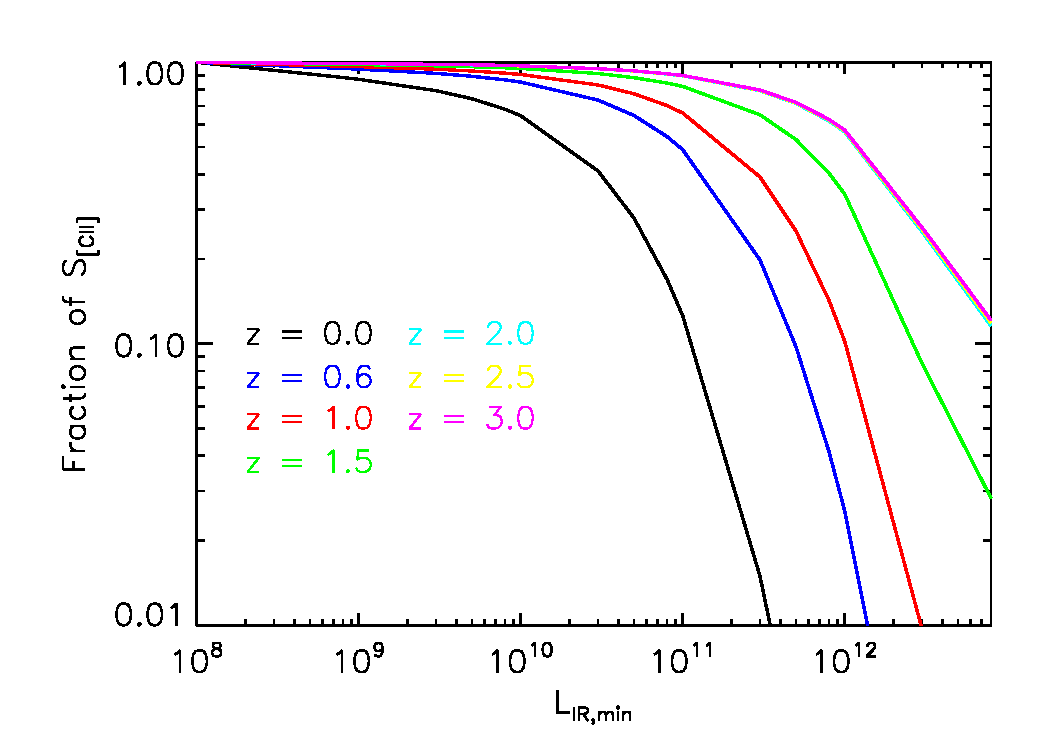
\includegraphics[width=0.45\textwidth]{fraction_cii_emissivity_vs_LIRmin_vs_z}
\caption{The fraction of total [CII] mean intensity as a function of lower limit in the luminosity function. Different color curves represent different redshifts, as labeled on the plot.}
\label{fig:frac_cii_b11_lirmin}
\end{figure}

\begin{figure}
\centering
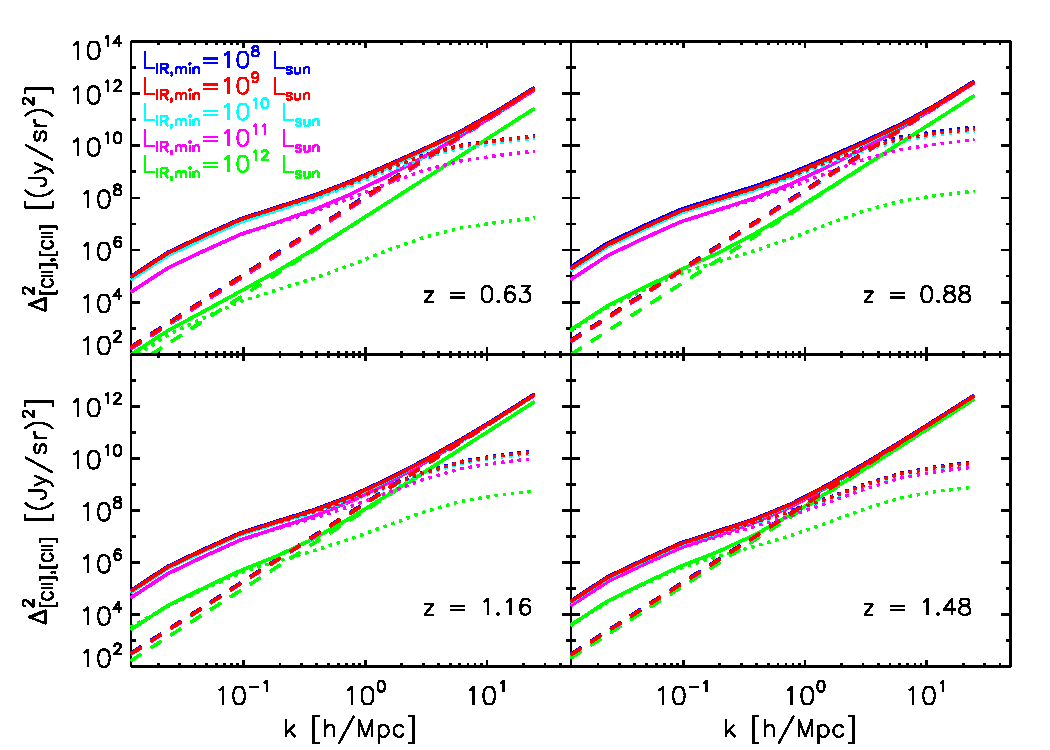
\includegraphics[width=0.45\textwidth]{pcii_STARFIRE_z63_z88_z116_z148_lirmin_halofit_bethermin_spinoglio_ap2p5m_1sqdeg_uhp_ktnonzero}
\caption{Predicted [CII] autocorrelation power spectra from $z = 0.63$ to $z = 1.48$. Blue, red, cyan, magenta, and green curves represent the power spectrum computed with a lower limit in the luminosity function corresponding to $10^8$, $10^9$, $10^{10}$, $10^{11}$, and $10^{12}$ L$_{\odot}$, respectively.}
\label{fig:pcii_lirmin}
\end{figure}

\section{The [CII] Power Spectrum}

\subsection{Observational Sensitivity to the Power Spectrum}

We present in this section an assessment of detectability of the [CII] power spectrum. In order to quantify the observational sensitivity, we adopt a realistic experimental platform with uninterrupted wavelength coverage in the redshift range of interest, namely, from 240 to 420 $\mu$m. This range is further divided into four bands to enable measuring redshift evolution in the signal. The width of each band has been set to span a redshift range of $\frac{\Delta{z}}{z_{center}} = 0.25$ to ensure there is no significant cosmological evolution within the band. Fiducial experimental parameters are summarized in Table ~\ref{tab:ExpParams}. The telescope aperture diameter, $D_{ap}$, and survey area, $A_{survey}$, are taken as 2.5 m and 1 deg$^2$, respectively, though we explore the effect of varying $D_{ap}$ and $A_{survey}$ on the signal-to-noise Ratio (SNR) (cf. Figure~\ref{fig:snr_nmode_k}).

\begin {table*}[t]
\begin{center}
\caption {Parameters for Envisioned Experimental Platforms} \label{tab:ExpParams} 
\begin{tabular}{ l c c c c}
\hline \hline
$D_{ap}$ (m) &\multicolumn{4}{c}{2.5} \\
$R = \lambda_{obs}/\Delta\lambda$ & \multicolumn{4}{c}{450} \\
N of Spectral Channels & \multicolumn{4}{c}{64} \\
N of Spectrometers (instantaneous spatial pixels) & \multicolumn{4}{c}{25} \\
$t_{obs}^{survey}$ (hr)&\multicolumn{4}{c}{450}\\
\hline
$z_{cen}$ for [CII] & 0.63 & 0.88 & 1.16 & 1.48 \\
Wavelength Range ($\mu$m) & 240-276 & 276-317 & 317-365 & 365-420 \\
$V_{voxel}$ (Mpc$^3$ h$^{-3}$) & 0.36 & 0.81 & 1.59 & 2.87 \\
$A_{pix}$ (Mpc$^2$ h$^{-2}$) & 0.044 & 0.096 & 0.19 & 0.35 \\
$\Delta$r$_{los}^{vox}$ (Mpc h$^{-1}$) & 7.8 & 7.8 & 7.7 & 7.5 \\
$\bar{S}_{\mathrm{[CII]}}$ (Jy sr$^{-1}$) & 4.56 $\times 10^3$ & 6.33 $\times$ 10$^3$ & 4.05 $\times 10^3$ & 2.55 $\times 10^3$ \\
\hline
\hline
 & \multicolumn{4}{c}{\emph{Atmospheric Balloon}}\\
$A_{survey}$ (deg$^2$) & 1 & 1 & 1 & 1 \\ 
$\sigma_N$ (10$^7$ Jy sr$^{-1}$ sec$^{1/2}$) & 3.4 & 2.1 & 1.5 & 1.0  \\
Line Sensitivity, $S_\gamma$ (10$^{-18}$ W m$^{-2}$ sec$^{1/2}$) & 15.8 & 11.3 & 9.20 & 7.10 \\
$f_{err}$ & 160 & 63 & 61 & 56 \\
\hline
 & \multicolumn{4}{c}{\emph{Cryogenic Satellite}} \\
$A_{survey}$ (deg$^2$) & 1,000 & 1,000 & 1,000 & 1,000 \\ 
$\sigma_N$ (10$^7$ Jy sr$^{-1}$ sec$^{1/2}$) & 0.030 & 0.034 & 0.039 & 0.043 \\
Line Sensitivity, $S_\gamma$ (10$^{-18}$ W m$^{-2}$ sec$^{1/2}$) & 0.139 & 0.185 & 0.240 & 0.306 \\
$f_{err}$ & 45 & 32 & 50 & 77 \\
\hline
\end{tabular}
\end{center}
\end{table*}

To define the survey depth, we adopt the quantity 

\begin{equation}
f_{err} \equiv \frac{\sigma_N}{\sqrt{t_{obs}^{vox}} \bar{S}_i}
\label{eq:ferr}
\end{equation}

which we call the fractional error. It is simply the inverse of the SNR on the mean intensity in a single voxel. Here $\sigma_N^2$ is the instrument sensitivity (noise equivalent intensity, or NEI, in units of Jy sr$^{-1}$ s$^{1/2}$, $\bar{S}_i$ is the mean intensity and $t_{obs}^{vox}$ is the observing time per voxel. (We take $i=\mathrm{[CII]}$ while the equations remain generally applicable to any line.) Error bar estimates and the total SNR for the power spectrum are calculated by assuming a spectrally flat noise power spectrum, so that the noise power in each voxel, $P_{N}$, is written as

\begin{align}
P_N & = \sigma_N^2 \frac{V_{vox}}{t_{obs}^{vox}} \\
& = \left(f_{err} \bar{S}_i \right)^2 V_{vox} \nonumber
\end{align}

where $\sigma_N^2$ is the instrument sensitivity (noise equivalent intensity, or NEI, in units of Jy sr$^{-1}$ s$^{1/2}$, $V_{vox}$ is the volume of a voxel, and $t_{obs}^{vox}$ is the time spent observing on a single voxel. The voxel volume is the product of pixel area, $A_{pix}$ (in units of comoving Mpc$^2$ h$^{-2}$), and the line of sight distance along a spectral channel, $\Delta$r$_{los}^{vox}$ (Mpc h$^{-1}$). $A_{pix}$ depends on the telescope aperture and observed wavelength according to $A_{pix} = (\lambda_{i,obs}/D_{ap}\times D_{A})^2$.

The variance of a measured $k$, $\sigma^2(k)$, is then written as

\begin{equation}
\sigma^2(k) = \frac{\left({P_{i,i}(k) + P_N(k)}\right)^{2}}{N_{modes}},
\end{equation}

where $N_{modes}$ is the number of wavemodes that are sampled for a given $k$ bin of some finite width $\Delta$log(k). (We have chosen $\Delta$log(k) = 0.3 for this analysis.)

The total SNR, in turn, is calculated from the expression 

\begin{equation}
SNR_{tot} = \sqrt{\sum_{bins} \left(\frac{P_{i,i}(k)}{\sigma(k)}\right)^2}
\end{equation}

The expected [CII] power spectrum, with corresponding predictions for SNR, at the same redshifts from Figure~\ref{fig:pcii_lirmin} are shown in Figure~\ref{fig:pcii_zall}. In calculating the power spectrum sensitivity for these power spectra, the two lowest line-of-sight modes and the lowest transverse mode are not included, since these modes will likely be compromised by the necessity of continuum foreground subtraction and beam-differencing in the fluctuation analysis. (The exact effect of continuum subtraction will need to be modeled via simulation.)

Table~\ref{tab:ExpParams} shows our instrument concepts.  We specify a 25-beam grating spectrometer covering the 240-420 $\mu$m band, each with 64 $R=450$ spectral channels operating near the photon background limit, illuminated with a 2.5-meter telescope. We consider a balloon experiment for which the photon background is due to 1\% emissivity in the atmosphere (a conservative average value) and 4\% in the telescope. A 450 hour integration (as might be obtained in a long duration balloon flight) over the 1 square degree with this system results in the $\sigma_N$, $f_{err}$, and line sensitivity values tabulated. We also consider a similar instrument on a cryogenic space-borne platform. The sensitivity in this case is obtained by specifying a detector sensitivity which adds $\sqrt{2}$ in quadrature to the noise in the photon background from the combination of zodiacal light, galactic dust, and a 6-K telescope with 4\% emissivity, similar to the proposed BLISS instrument for SPICA (e.g., see \citet{bradford12}). As the tabulated depths indicate, the space-born system is much more sensitive. Nevertheless, the balloon-borne experiment is capable of measuring the power spectrum with good sensitivity, and all error bars in this paper are based on the 450-hour balloon experiment, unless explicitly noted. 

\begin{figure*}[t]
\centering
\begin{tabular}{cc}
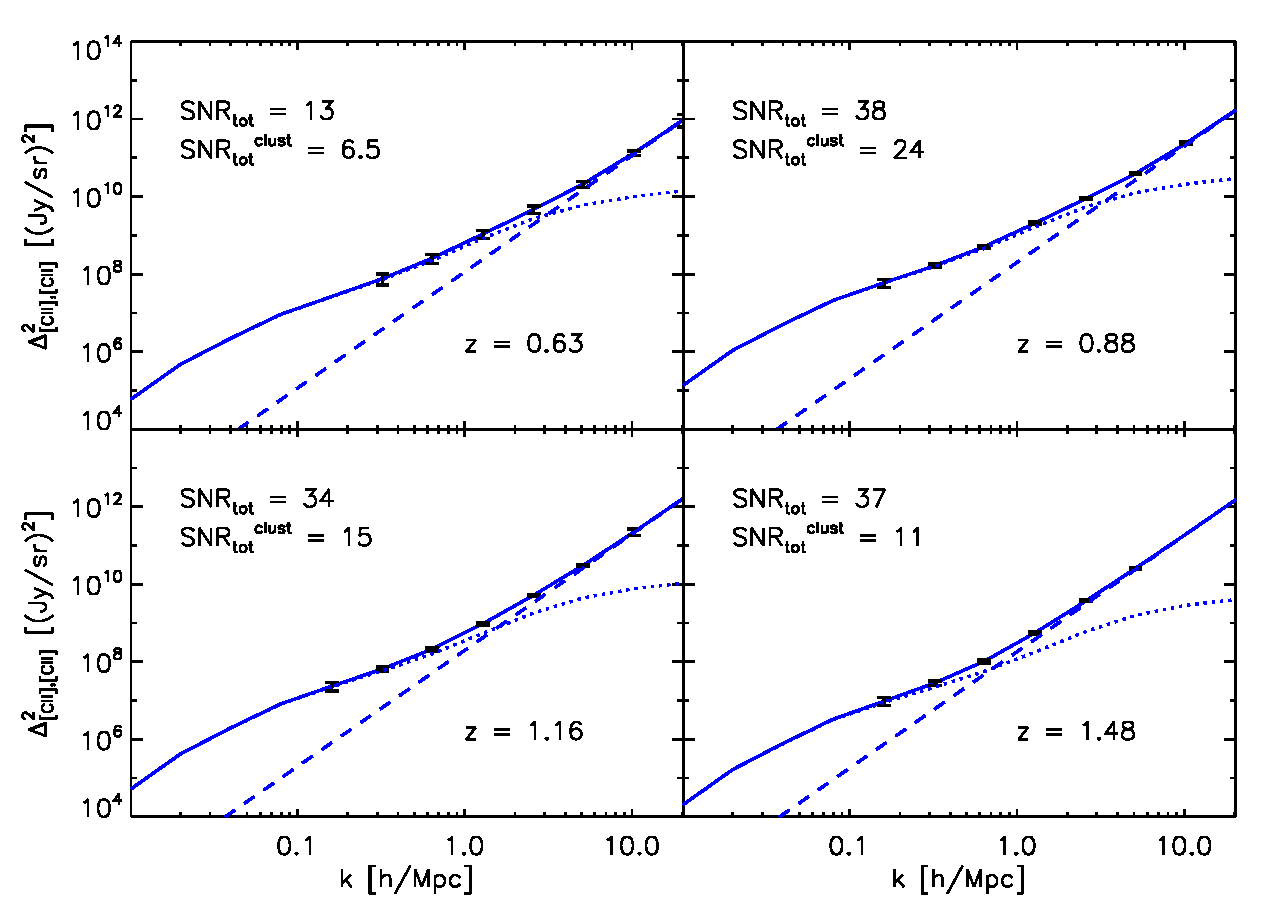
\includegraphics[width = 0.49\textwidth]{pcii_STARFIRE_z63_z88_z116_z148_halofit_bethermin_spinoglio_ap2p5m_1sqdeg_uhp_ktnonzero_minimaltext_450hr} &
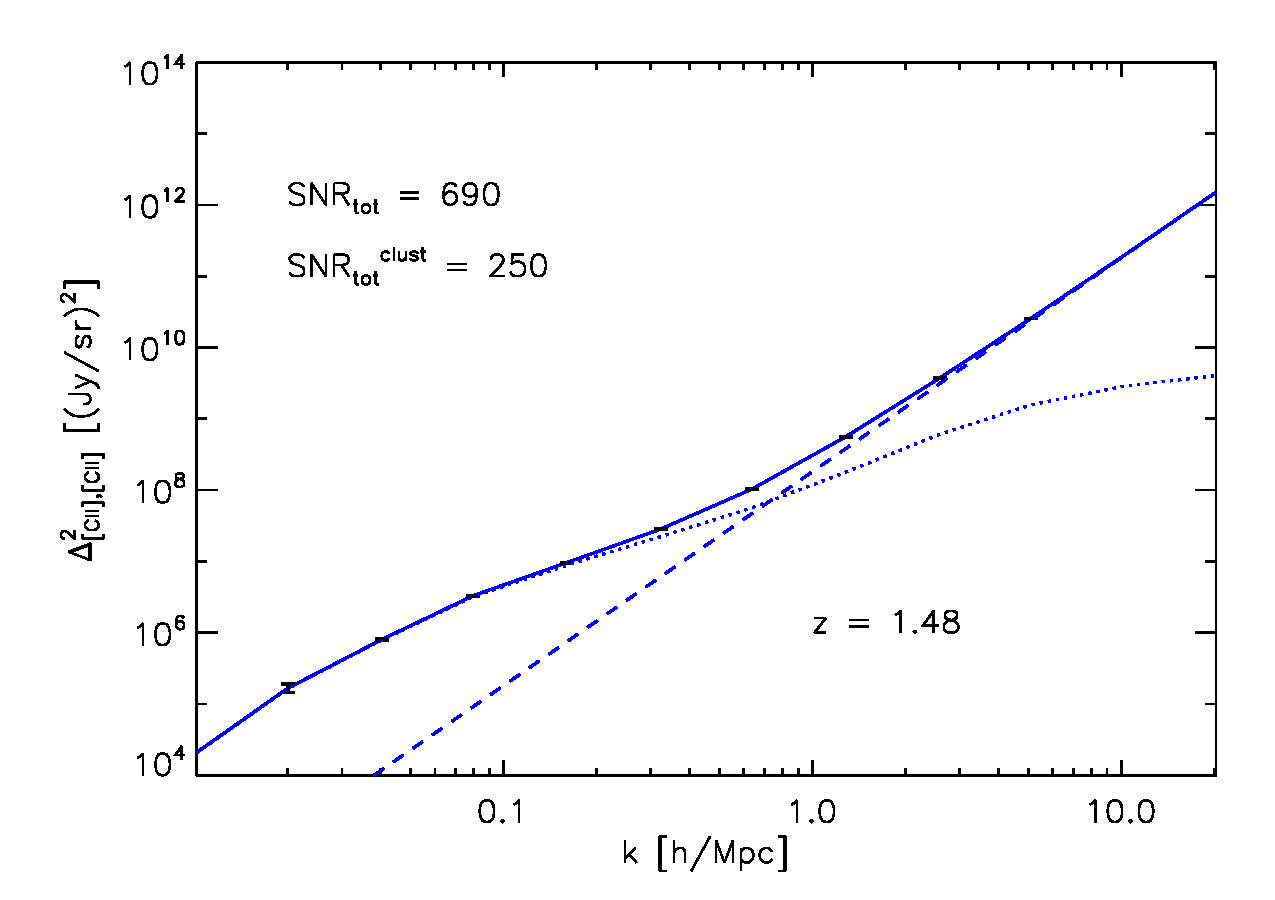
\includegraphics[width = 0.49\textwidth]{pcii_STARFIRE_z148_halofit_bethermin_spinoglio_ap2p5m_1000sqdeg_uhp_ktnonzero_minimaltext_450hr_space} \\
\end{tabular}
\caption{Left panel: Predicted [CII] power spectra with error bar estimates from $z$ = 0.63 to $z$ = 1.48 for the fiducial balloon experiment, and with a total observing time of 450 hours. Dotted curves indicate power from clustering (including contributions from linear and nonlinear terms), and dashed curves indicate the contribution from shot noise power. Right panel: [CII] power spectrum expected at $z=1.48$ with error bar estimates for the fiducial cryogenic satellite experiment.}
\label{fig:pcii_zall}
\end{figure}


We find that the total power spectrum, including power from both shot noise and clustering, is observable using the balloon platform with $\textrm{SNR}>10$ at all examined redshifts; the clustering power, in turn, can be detected with $\textrm{SNR}>10$ in the redshift range from $z = 0.88-1.48$. From space, it becomes feasible to survey larger areas ($\sim$1,000 deg$^2$) and maintain high SNR on the order of 100. (See Figure~\ref{fig:pcii_zall} for calculated SNRs.)

In Figures~\ref{fig:snr_asurvey} and \ref{fig:nmode_k} we examine the effect of changing the survey area and telescope aperture on SNR and accessible wavemodes, where the SNR has been plotted as as a function of survey area, and the number of modes has been plotted as a function of $k$. Our fiducial survey area of $A_{survey} = 1.0$ deg$^2$ for the balloon experiment is optimal for measuring as many large scale ($k\lesssim0.1$ h/Mpc) modes as possible with highest SNR in each $k$-bin; the square degree field is the approximate field size at which there are roughly equal contributions from cosmic variance and $P_N$, and larger areas do not improve SNR overall, or on individual modes of interest. By the same criterion, the field size for the space experiment at $z = 1.48$ becomes optimal for 1,000 deg$^2$. We do not consider surveys with areas less than a square degree because this prohibits measurement of power on large physical scales (cf. Figure~\ref{fig:nmode_k}).

\begin{figure}[b]
\centering
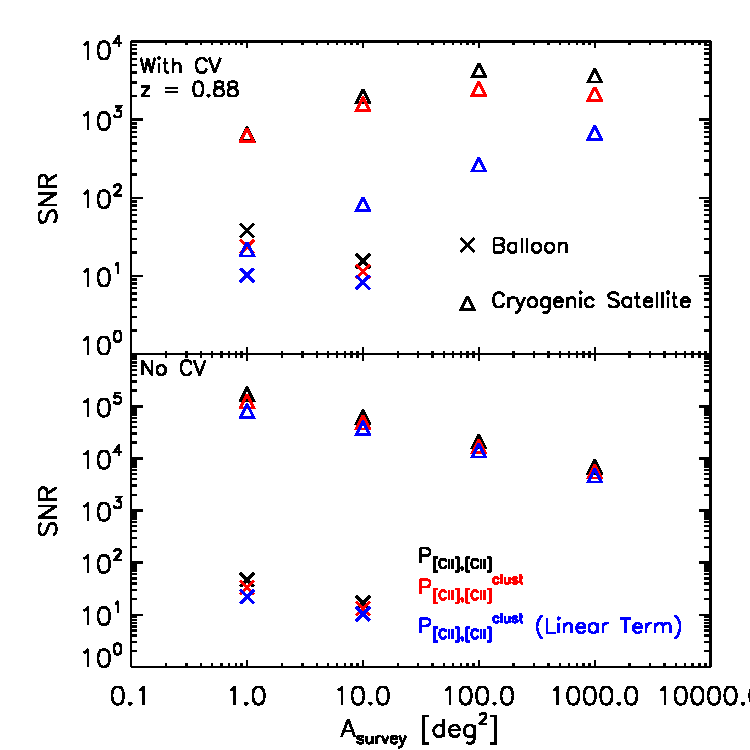
\includegraphics[width=0.45\textwidth]{snr_tot_clust_lin_asurvey_z88_450hr}
\caption{SNR on the total power spectrum (black), clustering power spectrum (red), and the linear portion ($k\lesssim0.1$ h/Mpc) of the clustering power spectrum (blue). Values for the balloon and cryogenic satellite experiments described in the text are designated with an ``X" and a triangle, respectively.}
\label{fig:snr_asurvey}
\end{figure}

\begin{figure}[h]
\centering
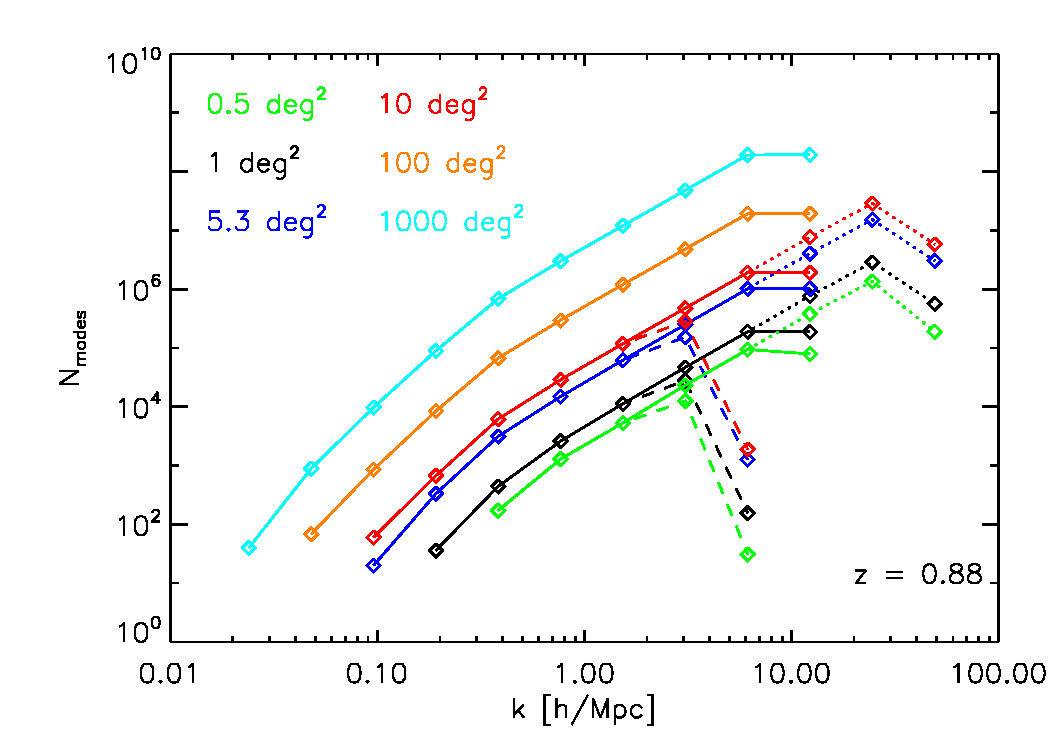
\includegraphics[width=0.45\textwidth]{nmode_vs_k_z88_100sqdeg_1000sqdeg}
\caption{Number of modes as a function of $k$ at $z=0.88$ for different survey areas. Telescopes with apertures yielding 0.1, 1, and 10 times the fiducial $V_{vox}$ are shown as the dotted, solid, and dashed lines, respectively.}
\label{fig:nmode_k}
\end{figure}

To better demonstrate how the observational parameters drive the behavior of SNR, we rewrite $P_N$ in terms of the parameters from Table 1 (where the units of $A_{survey}$ have been converted to physical area in units of Mpc$^{2}$ h$^{-2}$) giving 

\begin{equation}
\begin{split}
P_N& = \left(\sigma_N^2 A_{pix} \Delta r_{los}^{vox}\right) / \left({\frac{t_{obs}^{survey}}{n_{beams}/N_{instr}^{spatial}}}\right) \\
& = \left(\sigma_N^2 A_{pix}\Delta r_{los}^{vox}\right) /  \left(\frac{t_{obs}^{survey} N_{instr}^{spatial}}{A_{survey}/A_{pix}}\right)\\
& = \sigma_N^2 \frac{\Delta r_{los}^{vox} A_{survey}}{t_{obs}^{survey} N_{instr}^{spatial}}
\end{split}
\label{eq:pnoise}
\end{equation}

In this form, it becomes apparent that---with fixed number of spatial pixels, spectral resolution, and total observing time---the only factor driving up the amplitude of noise power is the survey area; the effect of increasing aperture only allows access to higher wavenumbers, which is important for subtracting the shot noise from the total power to reveal the clustering.

\subsection{Measuring $\bar{S}_{[CII]}(z)$}

As noted above, intensity mapping is naturally sensitive to the full range of galaxy luminosities through the mean intensity, which is imprinted in the linear (2-halo) clustering term. Shot noise must be accurately subtracted, and this should be straightforward given the high SNR in the shot-noise dominated k bins (Figure~\ref{fig:pcii_zall}).  Next, per Equation~\ref{eq:pclust}, it is necessary to divide out $P_{\delta,\delta}(k,z)$ and  $\bar{b}_{\textrm{[CII]}}^2(z)$.The confidence with which are \emph{a priori} known quantities becomes lower as $k$ increases. For example, the 1-halo power spectrum for DSFGs appears to be dependent on the IR luminosity of the contributing sources \citep{viero13}, indicating the need to map sufficiently wide areas that access $k$ modes where the power is largely independent of the level of 1-halo power. 

\begin{figure}[b]
\centering
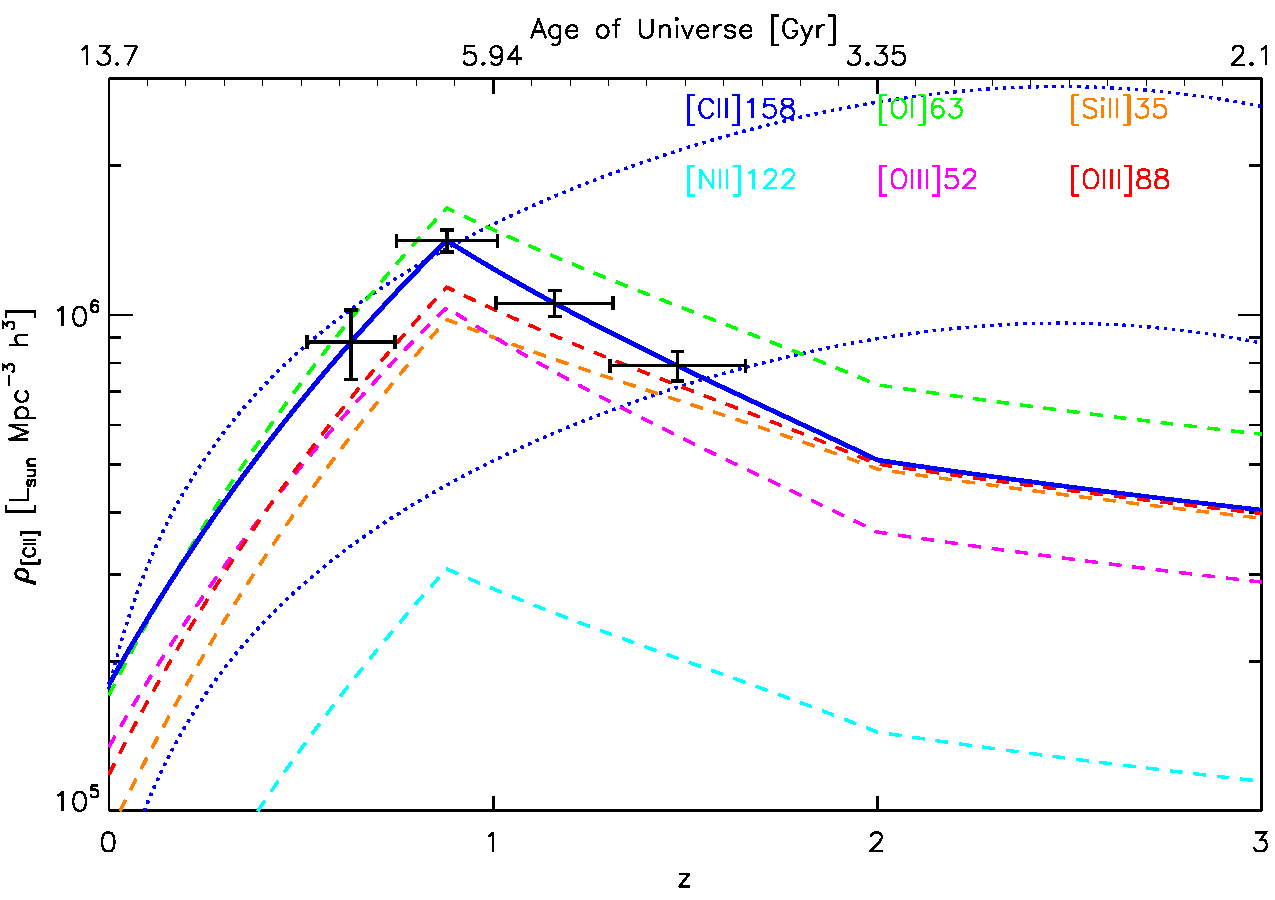
\includegraphics[width=0.45\textwidth]{s_cii_balloon_1sqdeg_450hr}
\caption{Error bar estimates on $\rho_{\textrm{[CII]}}$, as measured by the fiducial balloon experiment, at observed redshifts $z$ = 0.63, 0.88, 1.16, and 1.48. Errors in $z$ correspond to the redshift space spanned by the spectrometer bandwidth. The solid blue curve is the underlying model for [CII] luminosity density. The luminosity density of other bright IR lines are shown as the dashed colored curves, and the dotted curve is an estimate for $\rho_{\textrm{[CII]}}$ based on the fit to SFRD($z$) provided by \citet{hb06}, where we have used constant ratios of $L_{\textrm{[CII]}}$ to $L_{IR}$ equal to 0.001 (bottom curve) 0.003 (top curve) to convert from IR luminosity density to [CII] luminosity density.}
\label{fig:scii_z}
\end{figure}

Returning to Figure~\ref{fig:nmode_k}, we see that, for the purpose of measuring $\bar{S}_{\textrm{[CII]}}$ with the fiducial survey of 1 deg$^2$, there are two $k$ bins ($k = 0.16$ and 0.32 h/Mpc) in which the 2-halo clustering accounts for at least 80\% of the total power. (A survey with 10 deg$^2$, also shown in Figure~\ref{fig:nmode_k}, are wide enough to have three $k$ bins available in the linear regime, but the sensitivity on the additional mode with $t_{obs}^{survey}$= 450 hours is marginal.) Thus, in considering the case of $A_{survey} = 1.0$ deg$^2$, we find that it is possible to measure $\rho_{\textrm{[CII]}}(z)$ within $\sim10\%$ accuracy from $z = 0.63$ to $z=1.48$, as shown in Figure~\ref{fig:scii_z}, where the fractional uncertainty on $\bar{S}_{\textrm{[CII]}}(k,z)$ has been calculated as half the fractional uncertainty on $P_{\textrm{[CII],[CII]}}(k,z)$. In Figure~\ref{fig:scii_z}, we also include, for comparison, an estimate for $\rho_{\textrm{[CII]}}(z)$ based on the analytic fit to SFRD($z$) provided by \citet{hb06} and flat ratios of $L_{\textrm{[CII]}}/L_{IR} = 0.001$ and 0.003. (We use the standard relation between SFRD and infrared luminosity described in \citet{kennicutt98}.)

The cryogenic satellite offers an unprecedented platform for quantifying the evolution of far-IR line emission in cosmological volumes over time, with fractional uncertainties on the order of a tenth of a percent at each redshift for the 1,000 deg$^2$ survey ($t_{obs}^{survey} = 450$ hr).

\section{Observational Strategy: Comparing Intensity Mapping with Traditional Galaxy Surveys}

Now let us turn to a question regarding the motivation for intensity mapping in general, as well as in the specific case of [CII] at the redshifts relevant to this study. Having identified the galaxy redshift surveys as an alternative method to measure the mean intensity of the line-emitting galaxy population and to measure the 3D clustering power spectrum, it is natural to draw a comparison of the two approaches. 

The principal advantage of intensity mapping is that it naturally measures the mean intensity per equation~\ref{eq:intensity}, regardless of the shape of the luminosity function. Galaxy surveys always miss some of the light in the faintest galaxies, and this completeness problem is illustrated in Figure~\ref{fig:ngal_frac}. To make concrete comparisons in what follows we employ toy models for the infrared luminosity function (Figure~\ref{fig:schechterfuncs}) written in the Schechter formalism---parametrized by the usual $\alpha$, $L_*$, and $\phi_*$---and normalize the total IR luminosity density according to B11 (cf. Appendix for details). We stress that these Schechter models are not intended to represent a real interpretation of the distribution of galaxies, but are merely helpful for illustrating the effect of the LF \emph{shape} on the relative usefulness of intensity mapping and traditional galaxy surveys. In converting the IR LF to a line luminosity function, we use, in addition to the \citet{spinoglio12} relation for $L_{\textrm{[CII}}/L_{IR}$, a conservative and flat line-to-IR luminosity ratio of $10^{-3}$, relegating the luminosity-dependence of this ratio (and any redshift evolution) as a second order effect. 

\begin{figure}
\centering
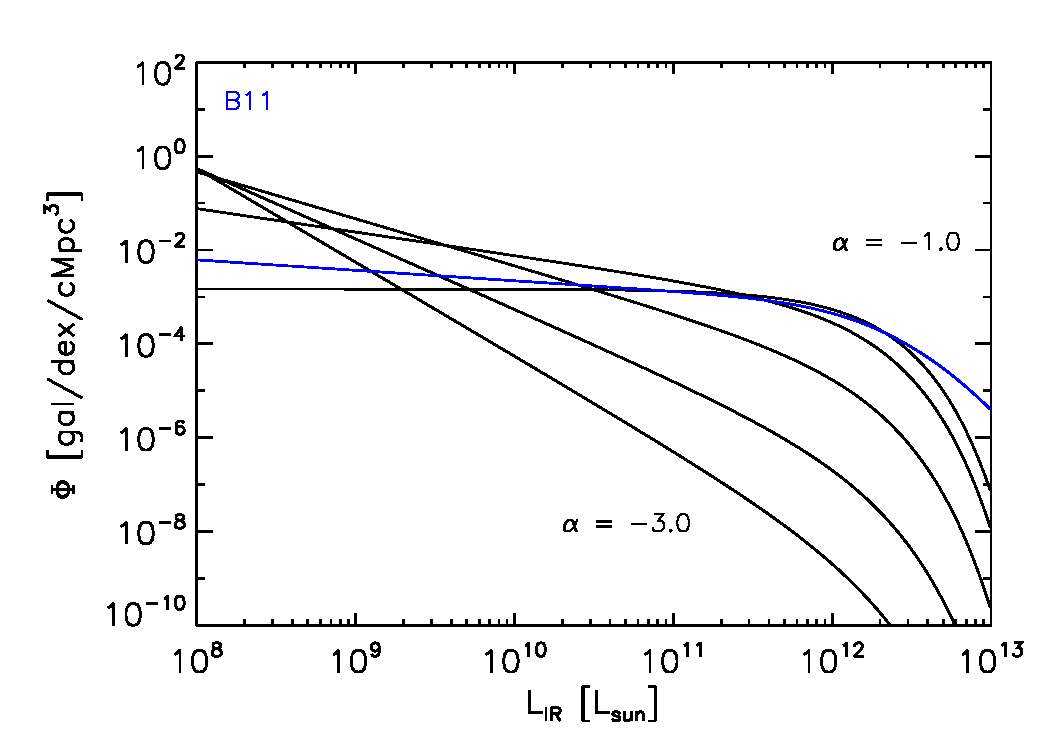
\includegraphics[width=0.5\textwidth]{phi_lir_schechter_bethermin11_Lstar1d12_Lmin1d8_Lmax1d13}
\caption{Toy model IR luminosity functions with faint-end slope (from top to bottom) $\alpha=-1.0, -1.5, -2.0, -2.5, -3.0$. The B11 model (blue curve) is plotted for comparison.}
\label{fig:schechterfuncs}
\end{figure}

\begin{figure}
\centering
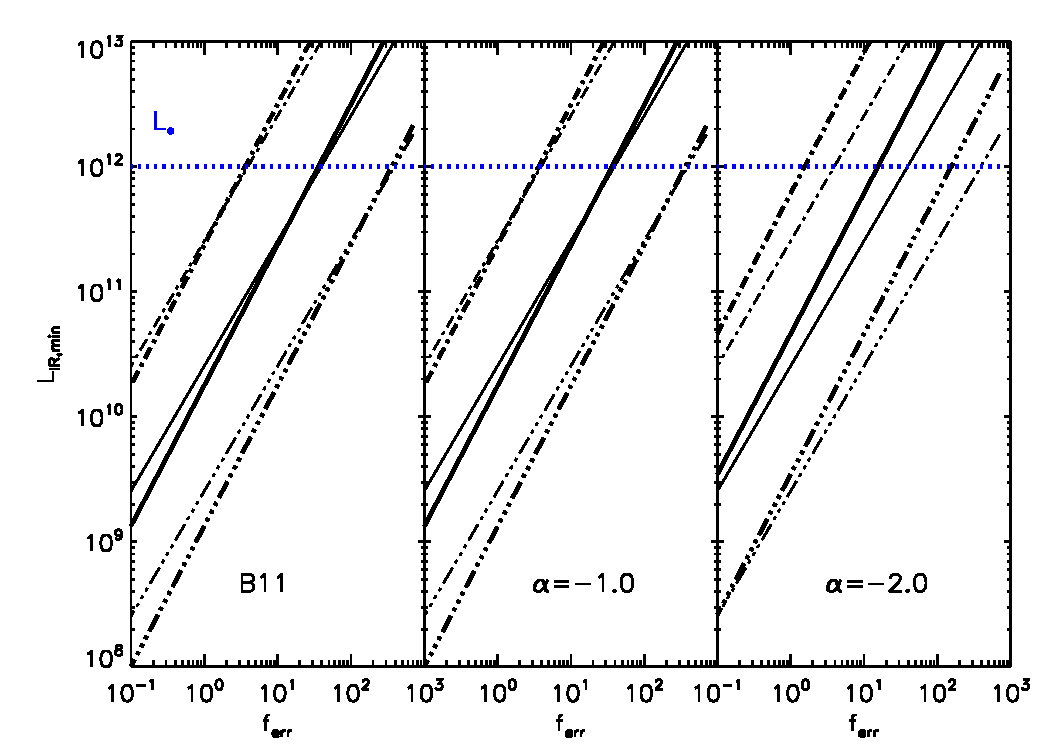
\includegraphics[width=0.5\textwidth]{lirmin_ferr_b11_alpham1p0_alpham2p0_lstar1d12}
\caption{IR depth as a function the fractional error. Results are plotted for the B11 (leftmost panel) model as well as the toy Schechter functions (remaining panels). Solid curves correspond to the fiducial aperture, $D_{ap}$ = 2.5 m. Dashed curves correspond to apertures scaled by a factor $\sqrt{\epsilon}$, where $\epsilon=10$ (triple-dot-dashed) and $\epsilon=0.1$ (dot-dashed). Thick curves correspond to our fiducial model for [CII] line intensity, based on Spinoglio fits, whereas thin curves denote the use of a constant ratio of $\frac{L_{\textrm{[CII]}}}{L_{IR}} = 10^{-3}$.}
\label{fig:lirmin_ferr}
\end{figure}

The line sensitivity, $S_{\gamma}$ (units of W m$^{-2}$ s$^{1/2}$), is the figure of merit for detecting an unresolved line in a point source, and we define individual detections at the $5\sigma$ level as having a flux above the instrumental noise in a voxel, i.e., above $5 \times S_{\gamma} t_{obs}^{vox}^{-1/2}$. (For this analysis, we safely assume the galaxy surveys have reliable spectroscopic redshifts and are not spatially confused. In reality, confusion can manifest when the density of sources is larger than the density of data voxels, ultimately raising the threshold for individual detection in a galaxy survey.) A convenient expression, which explicitly ties the minimum detectable line luminosity to a set of theoretical and experimental parameters, for the detection threshold can be written as

\begin{equation}
L_{i, min} = 5 \times f_{err} \rho_{i} V_{vox}, 
\label{eq:lirmin}
\end{equation}

Here, $f_{err}$ is the fractional error (Eq.~\ref{eq:ferr}) and $\rho_{i}$ is the comoving luminosity density of line $i$ at some $z$, or $L_*\phi_* \Gamma(2+\alpha, L/L_*)$ in the Schechter notation, so that equality holds between Equation~\ref{eq:lirmin} and the more conventional expression for the 5$\sigma$ detection threshold:

\begin{equation}
\frac{L_{i,min}}{4\pi D_L^2} \Leftrightarrow 5 \times S_{\gamma} t_{obs}^{vox}^{-1/2}
\end{equation}

The survey depths $L_{IR,min}$ as a function of $f_{err}$, $V_{vox}$, and $\alpha$ are plotted in Figure~\ref{fig:lirmin_ferr}. Note that we are investigating the effect of changing telescope aperture, which only changes the transverse dimensions of $V_{vox}$.

\begin{figure}
\centering
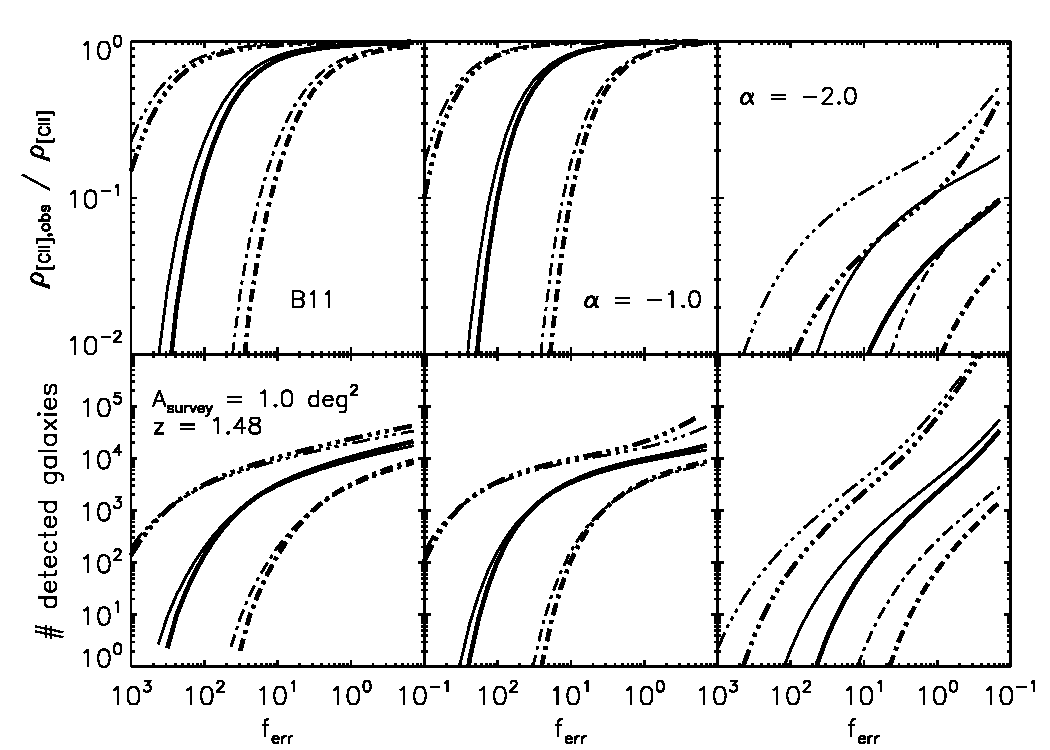
\includegraphics[width=0.5\textwidth]{Ngal_fracCII_STARFIRE_1sqdeg_z1p5_ferr_0p1vpix_vpix_10vpix_alpham1p0_alpham2p0_b11}
\caption{The observed fraction of [CII] luminosity density as a function of survey time for the square degree field and the predicted number of [CII]-detected galaxies . Results are plotted for the B11 (leftmost panel) model as well as the toy Schechter functions (remaining panels). Solid curves correspond to the fiducial aperture, $D_{ap}$ = 2.5 m. Dashed curves correspond to apertures scaled by a factor $\sqrt{\epsilon}$, where $\epsilon=10$ (triple-dot-dashed) and $\epsilon=0.1$ (dot-dashed). Thick curves correspond to our fiducial model for [CII] line intensity, based on Spinoglio fits, whereas thin curves denote the use of a constant ratio of $\frac{L_{\textrm{[CII]}}}{L_{IR}} = 10^{-3}$.}
\label{fig:ngal_frac}
\end{figure}

Since the intensity mapping technique contains information in the power spectrum from sources below a given $S_{\gamma}$, we expect that regimes in which the majority of galaxies are too faint to be resolved are better-suited for intensity mapping observations than observations via the traditional galaxy survey. Inspection of Equation~\ref{eq:lirmin} yields that this scenario occurs for large voxels (or large beam sizes), large fractional errors, or steep luminosity functions where the bulk of the galaxy number density is comprised of galaxies with sub-$L_*$ luminosities. These three limiting cases for the fiducial square degree survey at $z=1.48$ are illustrated in Figures~\ref{fig:ngal_frac} and \ref{fig:snr_vs_ferr} for the experimental goals of measuring mean intensity and the clustering power spectrum, respectively.

\begin{figure}[h]
 \centering
 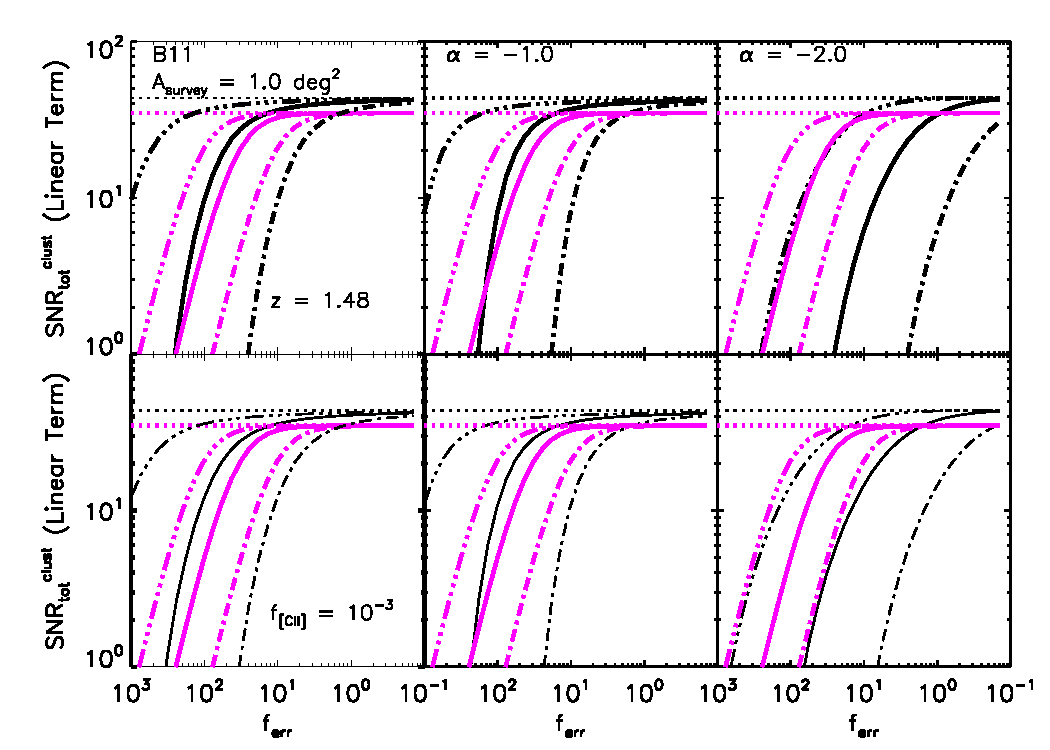
\includegraphics[width=0.5\textwidth]{snr_im_gs_ferr_nmodeIM_1d-1_1d3_b11_alpham1p0_alpham2p0_0p1vpix_vpix_10vpix_z148}
\caption{Total signal-to-noise ratio on the linear portion of the clustering power spectrum of [CII] at $z=1.48$ as a function of the fractional error. Results are plotted for the B11 (left panels) model as well as the toy Schechter functions (middle and right panels). $SNR_{IM}$ and $SNR_{GS}$ are plotted as the magenta and black curves, respectively. Solid curves correspond to the fiducial aperture, $d_{ap}$ = 2.5 m. Dashed curves correspond to apertures scaled by a factor $\sqrt{\epsilon}$, where $\epsilon=10$ (triple-dot-dashed) and $\epsilon=0.1$. The horizontal dotted line is the maximum SNR possible for each approach as set by the number of modes in the survey volume, which is lower for the intensity mapping experiment due to our described mode removal. Results are shown for predictions of [CII] intensity based on the Spinoglio fits (top panel) and a constant ratio of $\frac{L_{\textrm{[CII]}}}{L_{IR}} = 10^{-3}$ (bottom panel).}
\label{fig:snr_vs_ferr}
\end{figure}

As an example of the problem posed by steep luminosity functions for galaxy surveys aiming to measure the mean intensity, we find that for LFs with $\alpha$ of -1.5 (not shown) or -2.0, the galaxy surveys detect only 40\% and 3\% of the total [CII] light in integrating to an $f_{err}$ of 10. Increasing the telescope aperture by a factor of $\sqrt{10}$ (shown as the triple-dot-dashed curves) boosts this fraction to 60\% in the case of $\alpha = -1.5$, but still recovers 10\% or less of the $\rho_{\mathrm{[CII]}}$ for $\alpha = -2.0$. Note that an $f_{err}$ of 10 allows the galaxy survey to recover nearly 80\% of the total [CII] light at $z=1.5$ if $\alpha=-1.0$, but such a low fractional error requires either very low instrument noise or very long integration times---roughly $10^4$ hours for the fiducial instrument when observing a square degree field, for instance. (We refer the reader to Table~\ref{tab:ferrconvert} for the conversions between $f_{err}$ and integration time per voxel for the fiducial balloon experiment, as well as for the cryogenic satellite experiment.)
 
\begin {table*}[t]
\begin{center}
\caption {Conversions between $t_{obs}^{vox}$ and $f_{err}$ at $z = 1.48$} \label{tab:ferrconvert} 
\begin{tabular}{ l c c c}
\hline \hline
$t_{obs}^{vox} f_{err}^2$ ($\times 10^6$) & B11 & $\alpha = -1.0$ & $\alpha$ = -2.0 \\
\hline
Atmospheric Balloon & 1.54 & 1.57 & 2.83 \\
Cryogenic Satellite & 0.0286 & 0.0292 & 0.00526 \\
\hline
 \end{tabular}
 \end{center}
 \end{table}

The bottom row of Figure~\ref{fig:ngal_frac} breaks down the total emission in terms of the number of detectable galaxies. As is clear from comparison of panels in the top and bottom rows, a large sample of galaxies (of order 1,000 or greater) does not necessarily ensure an unbiased measure of the mean [CII] intensity. If, however, one extracts the aggregate, unresolved emission from [CII] via the intensity mapped power spectrum, one is essentially measuring $\frac{\rho_{\textrm{[CII]}, obs]}}{\rho_{\textrm{[CII]}}} = 1$ as soon as SNR on the linear clustering term of the power spectrum is sufficiently high, which was depicted in Figure~\ref{fig:scii_z}. 

There may be applications---such as measuring the BAO peak or searching for primordial non-Gaussianity in large-scale structure---for which the mean intensity is not required, and the shape of the power spectrum, rather than its absolute value, is of interest. For this application, we compare the SNR on a linear-term $k$ bin (up to $k < 0.3$ h/Mpc) for both galaxy detection and intensity mapping surveys (denoted, respectively, by the subscripts ``GS" and ``IM"), with the expressions:

\begin{align}
\mathrm{SNR}_{GS} & = \frac{\sqrt{N_{modes}} }{1 + 1/(\bar{b}_i^2P_{\delta,\delta}\bar{n}_{gal} )} \\
\mathrm{SNR}_{IM} & =  \frac{\sqrt{N_{modes}}}{1 + P_N/\left(\bar{S}_{i}^2\bar{b}_i^2P_{\delta,\delta}\right)} \\
 & = \frac{\sqrt{N_{modes}}}{1 + (f_{err}^2 V_{vox}) / (\bar{b}_i^2P_{\delta,\delta})} \nonumber
\end{align}

Even in this limited comparison of relative SNRs, the intensity mapping often outperforms galaxy surveys, as shown in Figure~\ref{fig:snr_vs_ferr}. For the steepest faint-end slope ($\alpha = -2.0$) we have tested, SNR$_{IM} >$ SNR$_{GS}$ for all $f_{err}$ and beam sizes (i.e., telescope apertures). For the flatter LFs, there are ranges of $f_{err}$ where SNR$_{IM} >$ SNR$_{GS}$ for the fiducial case, corresponding to when the galaxy surveys are shot-noise dominated. Figure~\ref{fig:contours} summarizes the results in Figure~\ref{fig:snr_vs_ferr}. It is important to remember that while surveys may detect a large number of galaxies, and thus attain appreciable SNR$_{GS}$ on the power spectrum, the sample of detected galaxies may not yield a measurement of mean intensity, for which a large fraction of the total [CII] light must be observed (cf. Figure~\ref{fig:ngal_frac}.) 

In considering only the SNR on the linear clustering term ($k<0.3$ h/Mpc) in our comparison, we do not address the potential of the 3D clustering power spectra to be used in the context of models which connect the host dark matter halos with their constituent galaxies by fitting to the observed 1-halo power. Since the 1-halo amplitude is highly sensitive to the luminosity of the contributing galaxy populations, we merely note in passing the potential of intensity mapping to constrain the distribution and types of galaxies within dark matter halos. 

\begin{figure}[H]
\centering
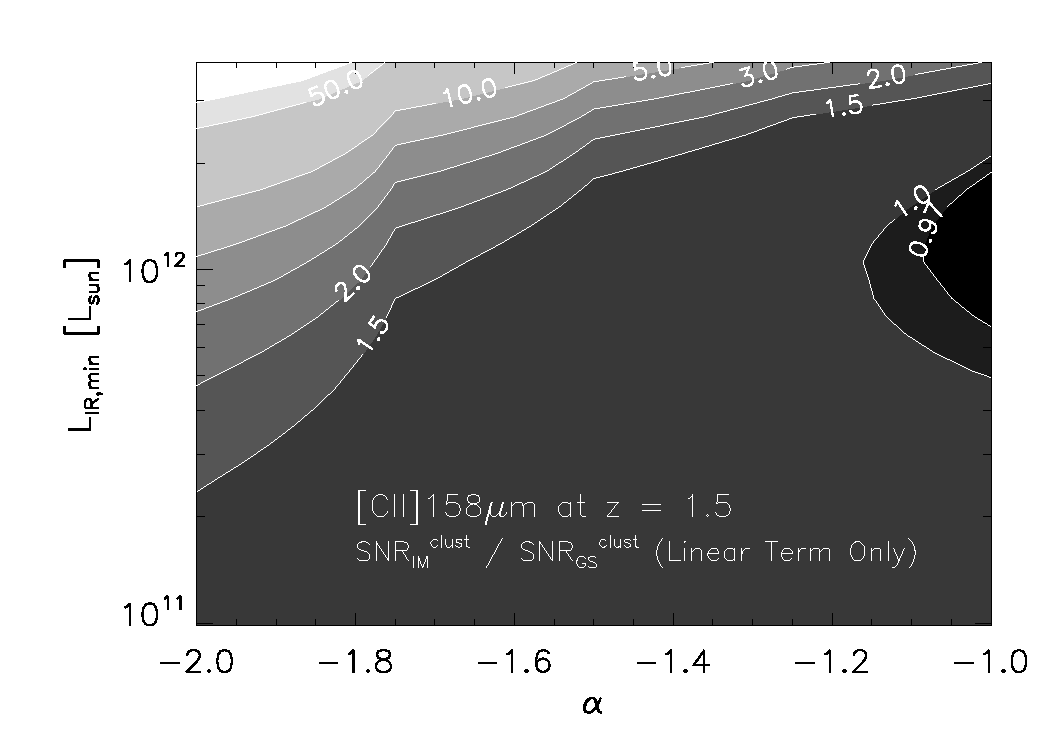
\includegraphics[width=0.5\textwidth]{contour_depth_alpha_cii_starfire}
\caption{Contours of SNR$_{IM}$/SNR$_{GS}$ for the linear term in the [CII] clustering power spectrum at $z = 1.5$, determined for a given depth (in $L_{IR}$) and IR LF faint-end slope $\alpha$.}
\label{fig:contours}
\end{figure}
 
\section{Summary and Outlook}

We have demonstrated the utility of the intensity mapping technique in measuring 3D power spectrum of bright FIR line emission at moderate redshifts, focusing on the important star-formation indicator [CII]. Fluctuations of FIR fine structure line intensities have been modeled by combining with the theorized dark matter power spectrum the empirically-constrained estimates of the IR luminosity from the B11 IR luminosity function and \citet{spinoglio12} line-to-$L_{IR}$ relations. We have presented predictions for the measurement of the [CII] auto-power spectrum between $0.63 < z < 1.48$, and found the power spectrum to be detectable in both clustering and shot noise terms in this redshift range with a modest, balloon-borne experimental platform, and exceptionally so with a more ambitious space-borne experimental platform. On large scales, the fact that the clustering amplitude of [CII] fluctuations is proportional to the mean [CII] intensity indicates the potential for measuring cosmic evolution of aggregate [CII], or of any target line, emission with the line intensity mapping approach. For the fiducial experiments considered in this paper, we have found that it would be possible to measure the [CII] luminosity density with fractional uncertainties on the order of 10\% or less. In examining the effect of luminosity function shape, telescope aperture, and fractional error (or instrument noise level) on the relative performances of intensity mapping to galaxy surveys, we have further demonstrated that, in the case where experiments with low fractional errors are not feasible, intensity mapping experiments often outperform galaxy redshift surveys when measuring the mean [CII] intensity. For steep luminosity functions, intensity mapping appears to be the only means of measuring average intensity and thus constraining the bulk of the luminosity function, as well as the optimal method of measuring the clustering power spectrum. 

Although beyond the scope of this paper, our findings here reinforce the notion that the $z > 6$ Universe presents an ideal landscape to learn about galaxy populations via intensity mapping. Strong evidence for steep ($\alpha \sim -2.0$) luminosity functions in the rest frame UV at $z\sim7$ \citep{bouwens14}, and larger voxels for a given aperture at higher redshifts, combine to position intensity mapping more favorably compared to galaxy surveys in probing the nature and clustering of the reionizing population. 

Looking to the future, the unprecedented sensitivity of background-limited spectrometer technology aboard space-borne experiments as described in this paper may become novel and important platforms to conduct large ($\sim 1,000$ deg$^2$) blind spatio-spectral surveys of FIR line emission, and warrants further study.
\\\\
The authors thank Adam Lidz and Olivier Dor\'{e} for useful discussions. BDU acknowledges support from the NASA GSRP Fellowship. 

\appendix

To explore the effect of the luminosity function shape on the relative performances of intensity mapping and galaxy surveys in observing the [CII] power spectrum and mean intensity of [CII] emitters, we have introduced toy models to represent different $\Phi(L_{IR}, z) \equiv \frac{\textrm{d}N}{\textrm{d}L_{IR}\textrm{d}V}$.

We parametrize our luminosity function as a Schechter function

\begin{equation}
\Phi(L_{IR},z) \textrm{d}L_{IR} = n_* \left(\frac{L_{IR}}{L_*}\right)^{\alpha} \exp\left(-\frac{L_{IR}}{L_*}\right) \textrm{d} \left(\frac{L_{IR}}{L_*}\right)
\end{equation}

where $n_*$ is the normalization for number density, $L_*$ is the characteristic luminosity at the knee, and $\alpha$ is the faint-end slope, as usual. 

Power-law luminosity functions are notoriously ill-behaved if the lower limit of integration for either the luminosity functions or its moments is extended to zero. Rather than implement a break in the power law, we simply cut it off at some $L_{IR, min}$ and choose to fix in our analysis the total IR luminosity density from galaxies as predicted by B11, denoted as $\rho_{IR}^{\textrm{B11}}$, such that

\begin{equation}
\int \textrm{d}\left(\frac{L_{IR}}{L_*}\right) n_* L_* \left(\frac{L_{IR}}{L_*}\right)^{\alpha+1} \exp\left(-\frac{L_{IR}}{L_*}\right) \equiv \rho_{IR}^{\textrm{B11}}
\label{eq:schechterlum}
\end{equation}

This is motivated by the observation that in many cases we do have constraints on the integrated light (from, for example, the cosmic infrared background or from the cosmic star formation rate density or the requirement of critical reionization), whereas we may not in general have detailed constraints on the distribution of light among galaxies, i.e., the shape of luminosity function.
 
The number density of sources, $n$, can, in turn, be computed from 

\begin{equation}
n = \int \textrm{d}\left(\frac{L_{IR}}{L_*}\right) n_* \left(\frac{L_{IR}}{L_*}\right)^{\alpha}\exp\left(-\frac{L_{IR}}{L_*}\right)
\end{equation}

Finally, equation~\ref{eq:schechterlum} allows us to calculate the [CII] luminosity density for each IR-normalized toy model as

\begin{equation}
\rho_{\textrm{[CII]}} = \int \textrm{d}\left(\frac{L_{IR}}{L_*}\right) n_* L_* \left(\frac{L_{IR}}{L_*}\right)^{\alpha+1} f_{\textrm{[CII]}} \exp\left(-\frac{L_{IR}}{L_*}\right) 
\end{equation}

where $f_{\textrm{[CII]}}$ is the fraction of IR luminosity emitted in [CII], or $\frac{L_{\textrm{[CII]}}(L_{IR})}{L_{IR}}$, described by the Spinoglio relations. Because $L_{\textrm{[CII]}}$ is slightly sublinear in $L_{IR}$, it follows that the toy models with steep faint-end slopes will produce more [CII] emission than their flatter counterparts. 



\bibliography{master_references}

\end{document}







